% To create a new appendix entry, add a new chapter and label to reference it 

\appendix
\appendixpage

\chapter{Dependencies}

\section{\textit{NPM} Dependencies} \label{appendix:dependencies}
\begin{itemize}
    \item @emotion/react@11.10.6
    \item @emotion/styled@11.10.6
    \item @microsoft/eslint-formatter-sarif@2.1.7
    \item @mui/material@5.11.13
    \item @playwright/test@1.31.2
    \item @testing-library/jest-dom@5.16.5
    \item @testing-library/react@13.4.0
    \item @testing-library/user-event@13.5.0
    \item @types/jest@27.5.2
    \item @types/node@16.18.16 
    \item @types/react-dom@18.0.11
    \item @types/react@18.0.28
    \item @typescript-eslint/eslint-plugin@5.56.0
    \item @typescript-eslint/parser@5.56.0
    \item axios@1.3.4
    \item eslint-plugin-react@7.32.2
    \item eslint@8.10.0
    \item mongodb@5.1.0
    \item playwright@1.31.2
    \item react-dom@18.2.0
    \item react-router-dom@6.9.0
    \item react-scripts@5.0.1
    \item react@18.2.0
    \item ts-md5@1.3.1
    \item typescript@4.9.5
    \item web-vitals@2.1.4
\end{itemize} 

\subsubsection{Dependency graph of npm package}
Example of a dependency graph for the npm package @playwright/test made from: \url{http://npm.anvaka.com/\#/view/2d/}

\begin{figure}[H]
    \centering
    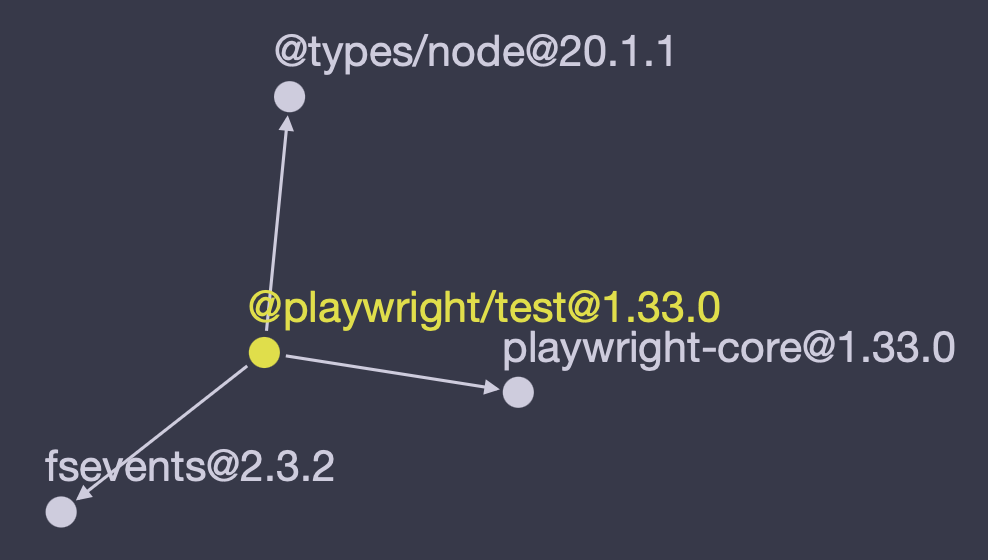
\includegraphics[width=10cm]{playwrightDependency.png}
    \caption{Playwright dependency graph}
    \label{fig:playwrightDependencies}
\end{figure}


\section{\textit{C\#} Application Dependencies} \label{appendix:CSharpdependencies}

\textit{MiniTwit.Core}
\begin{itemize}
    \item mapster
    \item Microsoft.AspNetCore.Mvc
    \item MongoDB.Bson
    \item MongoDB.Driver
\end{itemize}


\textit{MiniTwit.Infrastructure}
\begin{itemize}
    \item MongoDB.Driver
\end{itemize}

\textit{MiniTwit.Security}
\begin{itemize}
    \item Konscious.Security.Cryptography.Argon2
    \item Microsoft.Extensions.Options
\end{itemize}

\textit{MiniTwit.Server}
\begin{itemize}
    \item prometheus-net.AspNetCore  
    \item Serilog.AspNetCore    
    \item Serilog.Sinks.Grafana.Loki   
    \item Swashbuckle.AspNetCore 
\end{itemize}


\textit{MiniTwit.Tests/Infrastructure.Tests}
\begin{itemize}
   \item coverlet.collector 
   \item FluentAssertions  
   \item Microsoft.Extensions.Options   
   \item Microsoft.NET.Test.Sdk  
   \item Mongo2Go   
   \item Moq    
   \item xunit     
   \item xunit.runner.visualstudio  
\end{itemize}

\textit{MiniTwit.Tests/Server.Integration.Tests}
\begin{itemize}
   \item coverlet.collector 
   \item FluentAssertions  
   \item Microsoft.AspNetCore.Mvc.Testing    
   \item Microsoft.NET.Test.Sdk  
   \item Mongo2Go   
   \item xunit     
   \item xunit.runner.visualstudio  
\end{itemize}

\textit{MiniTwit.Tests/Server.Tests} 
\begin{itemize}
   \item coverlet.collector 
   \item Microsoft.AspNetCore.Mvc    
   \item Microsoft.NET.Test.Sdk  
   \item Moq   
   \item xunit     
   \item xunit.runner.visualstudio  
\end{itemize}


\section{CI/CD}
\label{appendix:CICDpdependencies}
\textit{build-latex.yml}
\begin{itemize}
    \item ubuntu-22.04
    \item actions/checkout@v3
    \item xu-cheng/latex-action@v2
    \item actions-js/push@master
\end{itemize}

\textit{build-test.yml}
\begin{itemize}
    \item ubuntu-20.04
    \item actions/checkout@v3
    \item actions/setup-dotnet@v3
    \item ubuntu-22.04
    \item actions/setup-node@v3
\end{itemize}

\textit{codeql.yml}
\begin{itemize}
    \item ubuntu-latest
    \item actions/checkout@v3
    \item github/codeql-action/init@v2
    \item github/codeql-action/autobuild@v2
    \item github/codeql-action/analyze@v2
    \item actions/upload-artifact@v2
\end{itemize}

\textit{continuos-deployment.yml}
\begin{itemize}
    \item ubuntu-latest
    \item actions/checkout@v3
    \item docker/setup-buildx-action@v2
    \item docker/login-action@v2
    \item docker/build-push-action@v4
    \item burnett01/rsync-deployments@5.2.1
    \item fifsky/ssh-action@master
\end{itemize}

\textit{eslint.yml}
\begin{itemize}
    \item ubuntu-latest
    \item actions/checkout@v3
    \item github/codeql-action/upload-sarif@v2
\end{itemize}

\textit{snyk-security.yml}
\begin{itemize}
    \item ubuntu-latest
    \item actions/checkout@master
    \item actions/setup-dotnet@master
    \item snyk/actions/setup@master
    \item actions/setup-node@master
    \item github/codeql-action/upload-sarif@v2 
\end{itemize}

\textit{sonarcloud.yml}
\begin{itemize}
    \item ubuntu-latest
    \item SonarSource/sonarcloud-github-action@de2e56b42aa84d0b1c5b622644ac17e505c9a049 
\end{itemize}

\section{Licenses of Direct Dependencies} \label{appendix:licenses_Dependencies}
\begin{itemize}
    \item MIT License
    \item BSD 2-Clause "Simplified" License
    \item BSD 3-Clause "New" or "Revised" License
    \item Apache License 2.0
    \item ISC License
    \item Creative Commons Attribution 4.0
    \item Creative Commons Zero v1.0 Universal
    \item Do What The F*ck You Want To Public License
    \item Unicode License Agreement - Data Files and Software (2016)
    \item W3C Software Notice and Document License (2015-05-13)
    \item BSD-4-Clause (University of California-Specific)
    \item IETF Contribution Agreement
    \item University of Illinois/NCSA Open Source License
    \item UNICODE, INC. LICENSE AGREEMENT - DATA FILES AND SOFTWARE
    \item zlib License
    \item Microsoft .Net Library
    \item Proprietary License
\end{itemize}
